%!TEX TS-program = xelatex
\documentclass[a4paper]{friggeri-cv}
\usepackage{afterpage}
\usepackage{hyperref}
\usepackage{color}
\usepackage{xcolor}
\usepackage{smartdiagram}
\usepackage{fontspec}


% if you want to add fontawesome package
% you need to compile the tex file with LuaLaTeX
% References:
%   http://texdoc.net/texmf-dist/doc/latex/fontawesome/fontawesome.pdf
%   https://www.ctan.org/tex-archive/fonts/fontawesome?lang=en
%\usepackage{fontawesome}
\usepackage{metalogo}
\usepackage{dtklogos}
\usepackage[utf8]{inputenc}
\usepackage{tikz}
\usetikzlibrary{mindmap,shadows}
\hypersetup{
    pdftitle={},
    pdfauthor={},
    pdfsubject={},
    pdfkeywords={},
    colorlinks=false,           % no lik border color
    allbordercolors=white       % white border color for all
}
\smartdiagramset{
    bubble center node font = \footnotesize,
    bubble node font = \footnotesize,
    % specifies the minimum size of the bubble center node
    bubble center node size = 0.5cm,
    %  specifies the minimum size of the bubbles
    bubble node size = 0.5cm,
    % specifies which is the distance among the bubble center node and the other bubbles
    distance center/other bubbles = 0.3cm,
    % sets the distance from the text to the border of the bubble center node
    distance text center bubble = 0.5cm,
    % set center bubble color
    bubble center node color = pblue,
    % define the list of colors usable in the diagram
    set color list = {lightgray, materialcyan, orange, green, materialorange, materialteal, materialamber, materialindigo, materialgreen, materiallime},
    % sets the opacity at which the bubbles are shown
    bubble fill opacity = 0.6,
    % sets the opacity at which the bubble text is shown
    bubble text opacity = 0.5,
}

\addbibresource{bibliography.bib}
\RequirePackage{xcolor}
\definecolor{pblue}{HTML}{0395DE}

\begin{document}
\header{Ali}{Heydari}
      {Computer Engineer}

% Fake text to add separator
\fcolorbox{white}{gray}{\parbox{\dimexpr\textwidth-2\fboxsep-2\fboxrule}{%
.....
}}

% In the aside, each new line forces a line break
\begin{aside}
  \includegraphics[scale=0.035]{img/Ali_Heydari.jpg}
  \section{Address}
Iran- Tehran- Narmak -
Iran University of Science and Technology.
    ~
  \section{Tel \& Skype}
   \href{tel:+989368563509}{+98 936 856 3509}
    ~
  \section{Mail}
 \href{mailto:ali4heydari@gmail.com}{\textbf{ali4heydari@}\\gmail.com}
    ~
  %\section{Web \& Git}
     %\href{https://github.com/ali4heydari}{github.com/ali4heydari}
    %\href{https://gitlab.com/u/ali4heydari}{gitlab.com/u/ali4heydari}
    %~
  % use  \hspace{} or \vspace{} to change bubble size, if needed
  \section{Programming}
    \textbf{Java}
\includegraphics[scale=0.40]{img/3stars.png}
    \textbf{C\#}
\includegraphics[scale=0.40]{img/3stars.png}
    \textbf{\LaTeX}
\includegraphics[scale=0.40]{img/4stars.png}
    \textbf{C++}
\includegraphics[scale=0.40]{img/2stars.png}
    \textbf{Android}
\includegraphics[scale=0.40]{img/2stars.png}
     \textbf{Python}
\includegraphics[scale=0.40]{img/2stars.png}
     \textbf{SQL}
\includegraphics[scale=0.40]{img/1stars.png}
     \textbf{C}
\includegraphics[scale=0.40]{img/1stars.png}
    ~
  \section{Skills}
       \smartdiagram[bubble diagram]{
         Design \\ 
        Pattern,
        Photoshop,
         TDD,
         \LaTeX,
          Primer,
        \textbf{Git}
       
        }
 ~
  \section{OS Preference}
    \textbf{Windows}
\includegraphics[scale=0.40]{img/5stars.png}
    \textbf{GNU/Linux}
\includegraphics[scale=0.40]{img/3stars.png}
%    \textbf{MacOS}
\includegraphics[scale=0.40]{img/1stars.png}
%    \textbf{Unix}
\includegraphics[scale=0.40]{img/2stars.png}
    ~
  \section{Places Lived}
    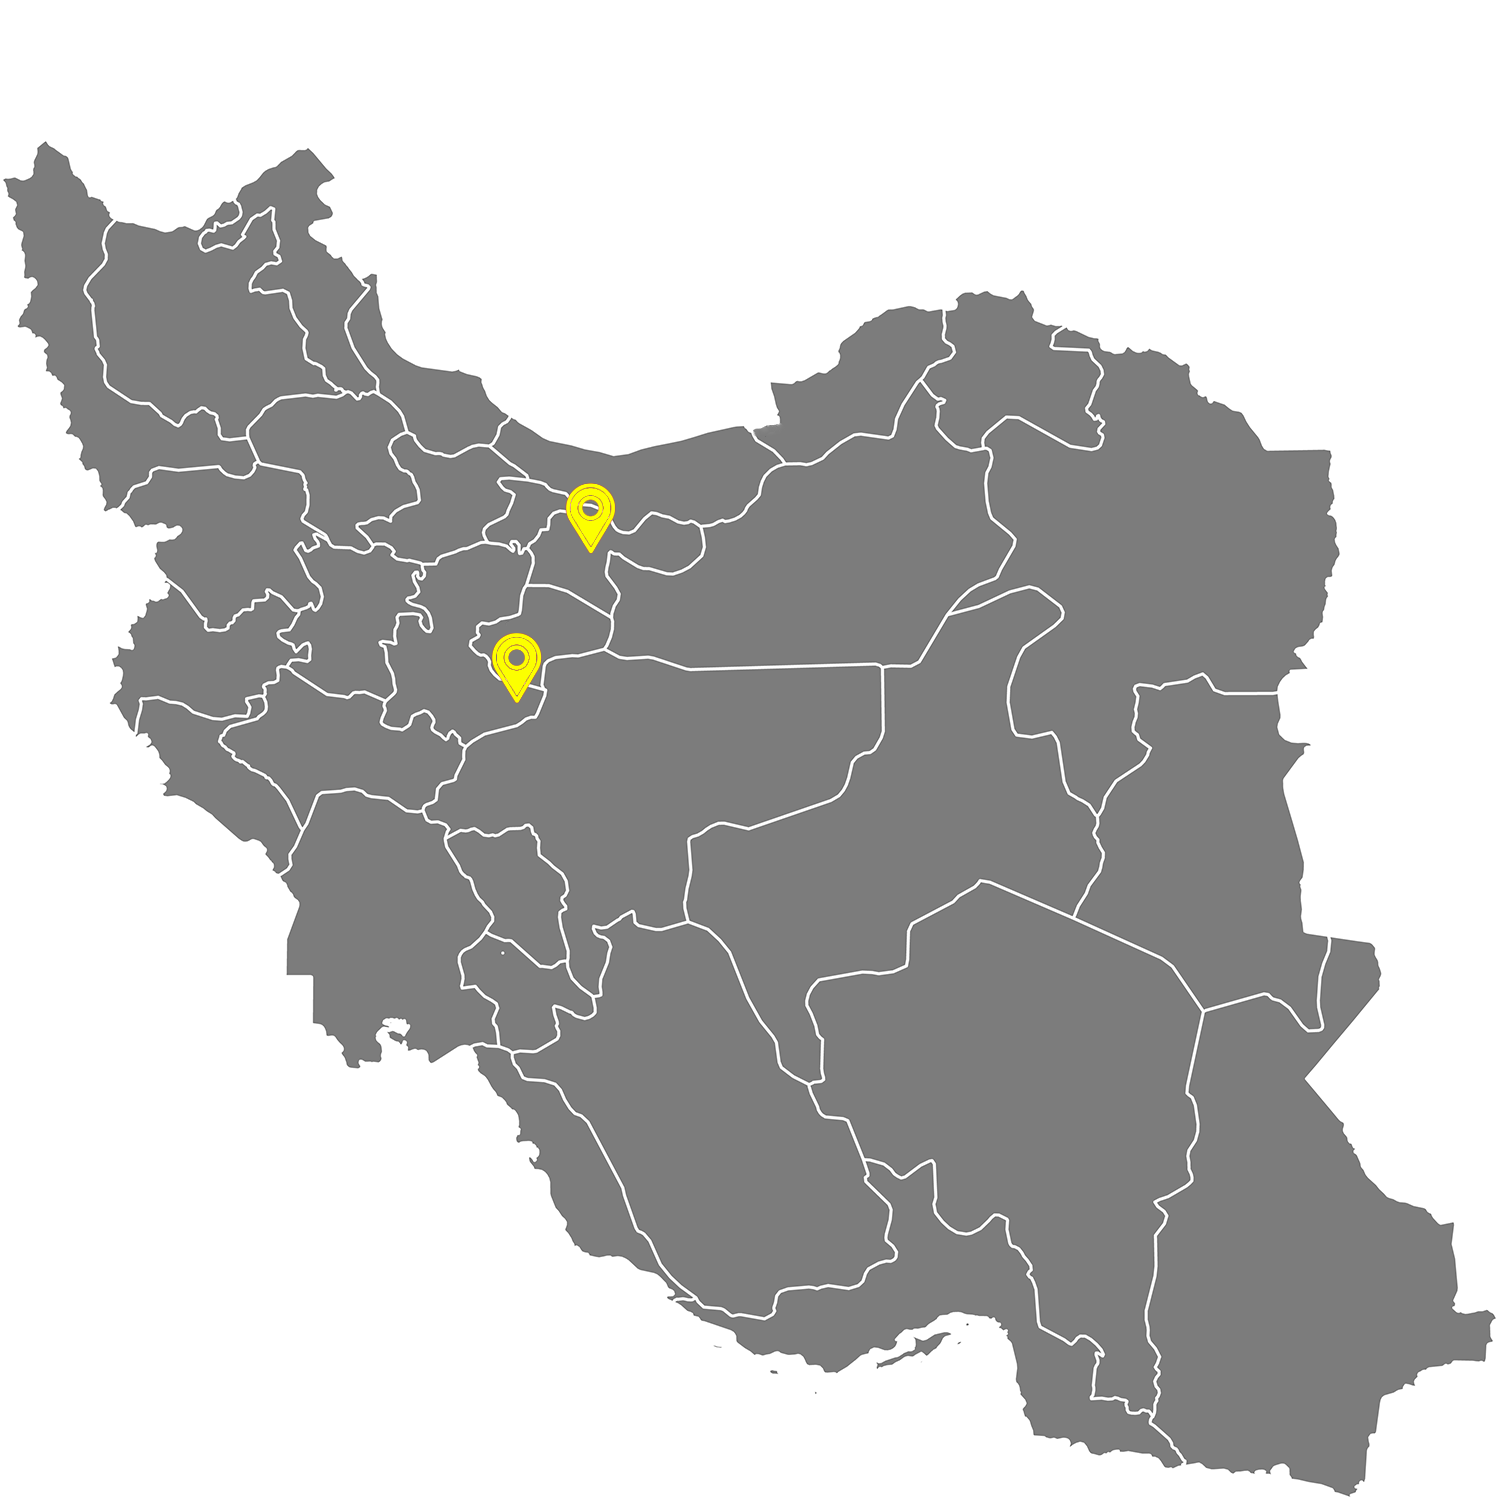
\includegraphics[scale=0.5]{img/iran.png}
    ~
%   \section{Languages}
  % \textbf{Persian}
\includegraphics[scale=0.40]{img/5stars.png}
   % \textbf{English}
\includegraphics[scale=0.40]{img/2stars.png}
   % ~
\end{aside}
~
\section{Experience}
\begin{entrylist}
  \entry
    {01/18-Now}
    {    Software Developer}
    {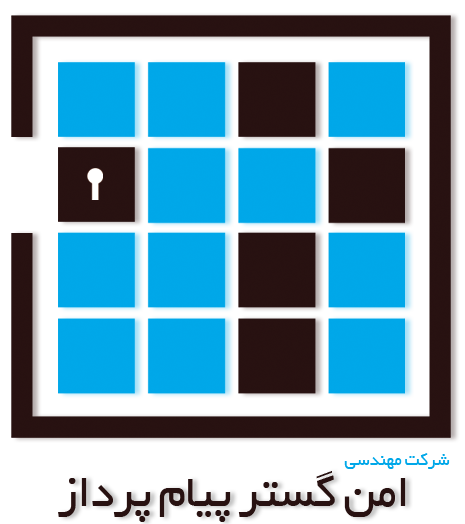
\includegraphics[scale=0.04]{img/AmnGostar_logo.png} AmnGostar Co}
    {Software developer for \emph{Sepehr} software project}
  \entry
    {10/17-04/18}
    {    Teacher \& course officer}
    {
\includegraphics[scale=0.005]{img/Kanoon_logo.png} Kanoon Farhangi Amoozesh}
    {Teacher \& course officer of physics and mathematics cousers}
  \entry
    {09/17-07/17}
    {   \emph{Tabesh} Cultural Group}
    {
\includegraphics[scale=0.03]{img/Tabesh_logo.jpg} Sharif University of Technology}
     {Member of the \emph{Tabesh} Cultural Group}
    \entry
    {09/17-07/17}
    {   Kimia Student Practical Group}
    {
\includegraphics[scale=0.03]{img/Kimia_logo.jpg} Sharif University of Technology}
    {Member of the \emph{Kimia} Student Practical Group}
    \entry
    {02/11-02/11}
    {    Calligraphy exhibition \emph{Noghte}}
    {
\includegraphics[scale=0.1]{img/Khoshnevisan_logo.png} Association of the Calligraphers of Delijan}
    {Participation in calligraphy exhibition \emph{Noghte}}
    \entry
    {02/08-06/10}
    {   Calligrapher}
    {
\includegraphics[scale=0.1]{img/Khoshnevisan_logo.png} Association of the Calligraphers}
    {Memmber of association of Calligraphers of Delijan}
\end{entrylist}
\\
\section{Education}
\begin{entrylist}
  \entry
    {2017 - Now}
    {     B.Sc in Computer Engineering}
    {
\includegraphics[scale=0.06]{img/IUST_logo_color.png}Iran University of Science and Technology}
    {}

  \entry
    {2016 - 2017}
    {    B.Sc in Chemical Engineering}
    {
\includegraphics[scale=0.015]{img/Sharif_logo.png} Sharif University of Technology}
    {}

  \entry
    {2011 - 2015}
    {    Scientific Disploma}
    {Beheshti Highschool}
  {}
\end{entrylist}

%\newpage

\section{Honors \& Awards}
\begin{entrylist}

      \entry
    {10/2015}
    {   Invention of \emph{Ghalamgir khoshnevisi}}
    {
\includegraphics[scale=0.06]{img/Ghovveh_logo.jpg} Iranian Patent Office}
    {Holds a patent for\\
    invention of \emph{Ghalamgir khoshnevisi}}

          \entry
    {10/2015}
    {   Invention of \emph{Damaban SAMA}}
    {
\includegraphics[scale=0.06]{img/Ghovveh_logo.jpg} Iranian Patent Office}
    {Holds a patent for \\
    invention of \emph{Damaban SAMA}}

              \entry
    {10/2015}
    {   Kharazmi Festival rank}
    {
\includegraphics[scale=0.06]{img/YKharazmi_logo.jpg} Iran Kharazmi Festival}
    {The first rank in the provincial section and the country's highest rank}

\end{entrylist}
\section{Certifications}
\begin{entrylist}
  \entry
    {02/2013}
    {Design Patterns}
    {
\includegraphics[scale=0.08]{img/Coursera_logo.jpg} Coursera -  
\includegraphics[scale=0.05]{img/UAlberta_logo.jpg} by University of Alberta}
    {}

    \entry
     {02/2013}
   {\emph{Momtaz} Degree}
    {
\includegraphics[scale=0.1]{img/Khoshnevisan_logo.png} Iran Calligraphers Association}
    {}
    
    \entry
     {02/2013}
   {Invention Authorization for \emph{Damaban SAMA}}
    {
\includegraphics[scale=0.09]{img/IROST_logo.jpg} IROST}
    {}
    
\end{entrylist}

\begin{flushleft}
\emph{August  2018}
\end{flushleft}
\begin{flushright}
\emph{Ali Heydari}
\end{flushright}

\end{document}
